\section{Analyze System Requirements}
\label{section:analyze-system-requirements}

OOSEM specifies externally observable behavior before tool selection \citep[Sec.~17.3.3]{friedenthal2014practical}. The Handbook distinguishes user and engineering levels and calls for concise, identified, verifiable obligations \citep[Sec.~I.4.1]{aguado2021cubesatse}. Observable conditions support qualitative and demonstration-based requirements as well as numerical ones.

\subsection{Scenarios and black-box functions}
{\small
\setlength{\tabcolsep}{4pt}
\setlength{\parskip}{0pt}
\setlength{\LTpre}{0.4\baselineskip}
\setlength{\LTpost}{0.4\baselineskip}
\renewcommand{\arraystretch}{1.06}
\begin{longtable}{@{}>{\raggedright\arraybackslash}p{\dimexpr0.14\linewidth-0.56\tabcolsep\relax}>{\raggedright\arraybackslash}p{\dimexpr0.52\linewidth-2.08\tabcolsep\relax}>{\raggedright\arraybackslash}p{\dimexpr0.34\linewidth-1.36\tabcolsep\relax}@{}}
\caption{Mission scenarios and exceptions.}\label{tab:framework-scenarios}\\
\toprule
\textbf{Scenario} & \textbf{Nominal service thread} & \textbf{Exceptional outcome} \\
\midrule
\endfirsthead
\caption[]{Mission scenarios and exceptions. (continued).}\\
\toprule
\textbf{Scenario} & \textbf{Nominal service thread} & \textbf{Exceptional outcome} \\
\midrule
\endhead
\bottomrule
\endfoot
SC01 / UC01 & Declare case/core adaptations. Write requirements and criteria. Bind sourced components, quantities and quotes to options. Run applicable analyses on a common basis. Review scoped evidence and retain engineer disposition. & Missing data, prices, criteria or model evidence remain gaps. Unsupported checks leave associated claims undetermined. Retain a reconstructable package. \\
SC02 / UC02 & Register a load, attitude, supply or software change. Identify reciprocal impacts on requirements, models, BOM, dictionaries and verification. Revise affected records, reassess claims and issue a reviewed successor. & Reject incompatible transfers and retain the previous baseline. Distinguish regenerated, stale and unresolved evidence. Expose unsupported targets and resource claims. \\
SC03 / UC03 & Retain failed-gate inputs and diagnostic variables. Check data quality, timing and model applicability. Propose updates, reassess affected claims and assemble the DUT/equipment, capture and safety proposal. & Calibration leaves intended-use validation separate. Missing limits, interfaces or safety review block physical readiness. Facility authorization remains external. \\
\end{longtable}
}
{\small
\setlength{\tabcolsep}{4pt}
\setlength{\parskip}{0pt}
\setlength{\LTpre}{0.4\baselineskip}
\setlength{\LTpost}{0.4\baselineskip}
\renewcommand{\arraystretch}{1.06}
\begin{longtable}{@{}>{\raggedright\arraybackslash}p{\dimexpr0.14\linewidth-0.28\tabcolsep\relax}>{\raggedright\arraybackslash}p{\dimexpr0.86\linewidth-1.72\tabcolsep\relax}@{}}
\caption{Black-box framework functions.}\label{tab:framework-functions}\\
\toprule
\textbf{Function} & \textbf{Observable service} \\
\midrule
\endfirsthead
\caption[]{Black-box framework functions. (continued).}\\
\toprule
\textbf{Function} & \textbf{Observable service} \\
\midrule
\endhead
\bottomrule
\endfoot
F01 & Guide users and tailor a controlled case. \\
F02 & Specify/revise requirements, criteria, decisions and dependencies. \\
F03 & Characterize/compare options with BOM, cost, RAM and resources. \\
F04 & Coordinate and reproduce analyses with declared applicability. \\
F05 & Define, map and check hardware, flight and ground service contracts. \\
F06 & Specify verification and assess safe later-execution readiness. \\
F07 & Control evidence, assess impacts and reconcile supplied observations. \\
F08 & Communicate justification and retain reviewed reusable lessons. \\
\end{longtable}
}

These are engineering services. EPS generation, charging, telemetry acquisition and recovery are modeled artifact behaviors. F04 consumes an identified ObservationPackage when comparing expected and observed signals. F06 consumes the RunPackage and applicable ModelCredibility record before assessing analytical evidence.

\subsection{Context and typed boundary interfaces}
\label{subsection:framework-context}

The context in Figure~\ref{fig:framework-context} is independent of vendor deployment. Candidate-native authoring and data services belong to their realization. Baseline custody remains framework responsibility even with external storage. Each exchange identifies source/revision, case/baseline, producer, dependencies, quantity/time meaning, provenance and status. A supported profile names tool versions, mapping, behavior and limitations.

\begin{figure}[!htbp]
\centering
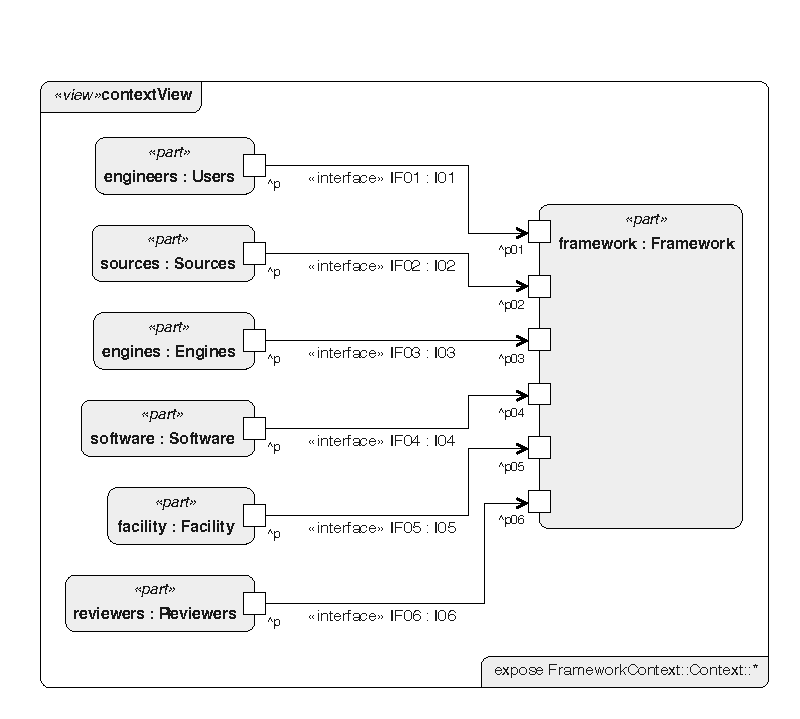
\includegraphics[width=\linewidth]{figures/sysml/context/sysml-defined-view-reportviews-contextview.pdf}
\caption{Framework boundary and six engineering exchange contracts.}
\label{fig:framework-context}
\end{figure}
{\small
\setlength{\tabcolsep}{4pt}
\setlength{\parskip}{0pt}
\setlength{\LTpre}{0.4\baselineskip}
\setlength{\LTpost}{0.4\baselineskip}
\renewcommand{\arraystretch}{1.06}
\begin{longtable}{@{}>{\raggedright\arraybackslash}p{\dimexpr0.22\linewidth-0.88\tabcolsep\relax}>{\raggedright\arraybackslash}p{\dimexpr0.42\linewidth-1.68\tabcolsep\relax}>{\raggedright\arraybackslash}p{\dimexpr0.36\linewidth-1.44\tabcolsep\relax}@{}}
\caption{Boundary types, ownership and failure behavior.}\label{tab:framework-boundary-contracts}\\
\toprule
\textbf{Interface} & \textbf{Actor/resource and exchanged types} & \textbf{Owner and checks} \\
\midrule
\endfirsthead
\caption[]{Boundary types, ownership and failure behavior. (continued).}\\
\toprule
\textbf{Interface} & \textbf{Actor/resource and exchanged types} & \textbf{Owner and checks} \\
\midrule
\endhead
\bottomrule
\endfoot
IF-01 Engineering use & PM, SE, EPS and non-EPS engineers. Needs, changes, criteria and decisions $\leftrightarrow$ guidance, models, impacts and justification. & L09/L02 check scope, identity and unresolved criteria. Incomplete submissions remain draft. Engineers authorize decisions. \\
IF-02 Knowledge/components & Suppliers, standards and literature. Datasheets, quotes and methods $\rightarrow$ sourced catalogue/assumptions. & L01/L04 check source, revision, units and applicability. Unsupported facts stay unknown. Supplier qualification is external. \\
IF-03 Discipline execution & Declared electrical, thermal, EMC, CAD, orbit, battery and RAM tools/operators. Controlled plan/inputs $\leftrightarrow$ raw results, environment, runtime and limits. & L05/L03 and L08 check profiles and transfer integrity. Preserve failure and unsupported/lossy mappings. No unsupported claim gets unqualified support. \\
IF-04 Software engineering & Flight/ground contributors and build environments. Dictionaries, commands/modes and target profiles $\leftrightarrow$ mappings, builds and resource evidence. & L03 checks versions and typed or message semantics. Missing implementation/target evidence stays unresolved. Mission functionality remains an artifact. \\
IF-05 Facilities/evidence & Technician, safety authority and later instruments/DUTs. Proposal/capture contract $\leftrightarrow$ profiles, dispositions and observations. & L07 checks safety/procedure completeness. L06 checks clocks/channels/validity. Preserve invalid samples/masks. Incomplete readiness stays blocked. \\
IF-06 Review/evaluation & Reviewer/researcher/reproducer. Requests, reference answers and findings $\leftrightarrow$ packages, replay, views and observations. & L09/L05 identify subject and rule. Missing dependencies and contested findings remain explicit. Project assessment has separate authority. \\
\end{longtable}
}

\subsection{Expected variation and design constraints}

Load schedules, operating modes, component selections, prices and failure assumptions can change. Solver versions, software mappings and later facility interfaces can also change. Their frequencies are unknown. Versioned profiles and explicit field ownership isolate these changes. The common core and allowed case adaptations are fixed before evaluation. A core change requires a successor baseline and both case reruns \citep[Sec.~17.3.3]{friedenthal2014practical}.

The current problem definition leaves vendor and repository choices open. It supplies no hard budget. Requirements, modeling and analysis may be framework capabilities or checked integrations. SysML v2 describes this OOSEM study. Candidate implementations retain their native languages and tools. Access, export rights and resource feasibility remain candidate verification obligations.

\subsection{Control and critical-property protocols}

Reject or quarantine incompatible identifiers, dimensions, units, signs, time and mode meanings before registration. Preserve raw submissions and accepted content. Changes are reviewed proposals. Successors retain previous revisions, failed-gate context and affected evidence status. Execution, trace completeness, model applicability and verification verdict are separate. An unresolved critical finding blocks an unqualified supported claim. A successor alone is not a correct completed change.

Retain raw observations, sample/receipt times, active-unit/mode context and masks. Missing or inactive readings are not zero. Calibration creates a proposed parameter revision. Validation uses separately identified evidence. A physical proposal needs limits, equipment/DUT interfaces, hazards, fault envelope, isolation, abort/recovery and safety-review status. The facility alone authorizes work. A case-two core repair requires a new baseline and both reruns.

MOPs observe framework behavior and contribute to the matching MOEs. Numerical rules are profile-specific and remain open where unsupported. Table~\ref{tab:framework-mop-protocols} groups their protocols. Detailed task definitions and original-measure crosswalks remain in the registry.
{\small
\setlength{\tabcolsep}{4pt}
\setlength{\parskip}{0pt}
\setlength{\LTpre}{0.4\baselineskip}
\setlength{\LTpost}{0.4\baselineskip}
\renewcommand{\arraystretch}{1.06}
\begin{longtable}{@{}>{\raggedright\arraybackslash}p{\dimexpr0.23\linewidth-0.46\tabcolsep\relax}>{\raggedright\arraybackslash}p{\dimexpr0.77\linewidth-1.54\tabcolsep\relax}@{}}
\caption{Critical-property observation protocols. All numbers have the MOP- prefix.}\label{tab:framework-mop-protocols}\\
\toprule
\textbf{MOP group} & \textbf{Protocol} \\
\midrule
\endfirsthead
\caption[]{Critical-property observation protocols. All numbers have the MOP- prefix. (continued).}\\
\toprule
\textbf{MOP group} & \textbf{Protocol} \\
\midrule
\endhead
\bottomrule
\endfoot
MOP-01, 03, 06, 08 & Qualified references for requirement quality, BOM/cost arithmetic, RAM transformations, both software mappings and command/recovery behavior. Preserve missing prices, rates and target evidence. \\
MOP-02 & Blind discrepancy and clean fixtures for semantics, traces, impacts, stale and interrupted changes. Report TP, FP, FN by family and critical misses. \\
MOP-04, 09 & Pin models, solvers, inputs, environment and criteria. Retain raw histories, coupling/runtime and independent replay under fixed result-specific tolerances. \\
MOP-05, 07 & Exercise in-domain/extrapolated claims, calibration updates, noise, skew, gaps and inactive samples. Compare residuals/masks with references. Agree applicability and timing limits. \\
MOP-07, 10, 11 & Technician/reviewer tasks, clean installation and two frozen-core cases. Retain omissions, errors, clarification, person-hours, footprint and dated direct-cost evidence. \\
\end{longtable}
}

\subsection{Verifiable framework requirement leaves}
\label{subsection:framework-requirements}

All forty obligations and mission parents follow. I is inspection, A analysis, D demonstration and T test. V01--V40 verify the same-numbered FR. Every procedure is planned. The structured registry specifies all forty fixtures, conditions, stimuli, expected responses, acceptance observations and evidence once. No passed verdict is asserted. A not-applicable field requires rationale.
{\small
\setlength{\tabcolsep}{4pt}
\setlength{\parskip}{0pt}
\setlength{\LTpre}{0.4\baselineskip}
\setlength{\LTpost}{0.4\baselineskip}
\renewcommand{\arraystretch}{1.06}
\begin{longtable}{@{}>{\raggedright\arraybackslash}p{\dimexpr0.2\linewidth-0.8\tabcolsep\relax}>{\raggedright\arraybackslash}p{\dimexpr0.68\linewidth-2.72\tabcolsep\relax}>{\raggedright\arraybackslash}p{\dimexpr0.12\linewidth-0.48\tabcolsep\relax}@{}}
\caption{Framework leaves, mission derivation and planned verification.}\label{tab:framework-requirements}\\
\toprule
\textbf{Leaf / MR parents} & \textbf{Obligation} & \textbf{V / method} \\
\midrule
\endfirsthead
\caption[]{Framework leaves, mission derivation and planned verification. (continued).}\\
\toprule
\textbf{Leaf / MR parents} & \textbf{Obligation} & \textbf{V / method} \\
\midrule
\endhead
\bottomrule
\endfoot
FR-01\par MR-01, MR-02 & The framework shall retain each requirement as an identified record with source need, parent, rationale, observable quantities or conditions and applicable units, owner, verification method, criterion, and resolution status. A not-applicable field shall retain its rationale. & V01\par I, T \\
FR-02\par MR-01, MR-11 & The framework shall provide requirement and traceability templates, worked EPS examples, and a guided reference workflow that covers writing criteria, linking evidence, and interpreting gaps. & V02\par I, D \\
FR-03\par MR-01, MR-07, MR-11 & The framework shall retain a source-linked catalogue of requirement derivation and verification methods, standards, and activity templates with applicability, tailoring rationale, and limitations. & V03\par I, D \\
FR-04\par MR-02, MR-10 & The framework shall retrieve applicable links from needs and requirements to design decisions, model inputs, verification criteria and results, and retrieve the reverse paths. & V04\par T \\
FR-05\par MR-02, MR-03, MR-08 & The framework shall identify the requirements, EPS and non-EPS allocations, BOMs, models, software definitions, procedures, and evidence affected by a designated change. & V05\par A, T \\
FR-06\par MR-02, MR-05, MR-07 & The framework shall issue a successor baseline for an accepted change that retains its request and failed-gate context and marks affected evidence as regenerated, stale, or unresolved. & V06\par T \\
FR-07\par MR-02, MR-09 & The framework shall retain identified, retrievable baselines of engineering records, case configuration, and evidence with revision history and distinct identities for accepted successors. & V07\par T \\
FR-08\par MR-02, MR-09 & The framework shall check transferred identifiers, structure, quantities, units, polarity, time bases, interface meanings, and provenance against a declared contract and retain explicit rejection findings. & V08\par T \\
FR-09\par MR-02, MR-05, MR-09 & The framework shall associate each result with its producer, method, requirement and decision, design and hardware configuration, software and model versions, parameter set, input data, environment, and raw output. & V09\par I, T \\
FR-10\par MR-09 & The framework shall provide controlled instructions and dependencies to reconstruct and execute a designated analysis and compare its raw outputs using declared result-specific rules and tolerances. & V10\par D, T \\
FR-11\par MR-02, MR-05, MR-10 & The framework shall report missing, rejected, stale, out-of-domain, failed, and unresolved evidence with its affected claim, criticality rationale, owner and disposition. & V11\par T \\
FR-12\par MR-03 & The framework shall generate and revise a candidate-specific BOM from identified physical design items with assembly, quantities, part identifiers, variant and selection status, and source revision. & V12\par A, T \\
FR-13\par MR-03 & The framework shall derive a revision-linked financial estimate from the BOM and declared additional cost categories while retaining price source, date, currency, quantity, estimate basis, uncertainty and missing data. & V13\par A, T \\
FR-14\par MR-03, MR-04 & The framework shall produce a comparison of designated EPS architectures using a common requirement, assumption, evidence and criterion basis with feasibility status, raw measures, uncertainty and decision rationale. & V14\par A, T \\
FR-15\par MR-04, MR-11 & The framework shall provide a configurable generic EPS representation covering requirements, functions, logical and physical elements, interfaces, modes and states, with case-specific parameter and extension records. & V15\par I, D \\
FR-16\par MR-04, MR-05, MR-08 & The framework shall compose time-dependent subsystem demand, duty cycles, schedules and mode transitions with orbit, attitude, irradiance, eclipse, thermal conditions and EPS supply and protection behavior. & V16\par A, T \\
FR-17\par MR-01, MR-02, MR-04 & The framework shall record how sourced component power and thermal characteristics and subsystem behavior become EPS or component requirement parameters, including units, uncertainties, allowable ranges and criterion decisions. & V17\par A, T \\
FR-18\par MR-04, MR-07 & The framework shall exchange identified EPS component and design data with declared electrical, thermal, EMC and CAD analysis tools and retain model mappings, applicable outputs and unsupported checks. & V18\par D, T \\
FR-19\par MR-04, MR-07 & The framework shall execute or coordinate declared virtual EPS and component verification scenarios for dynamic loads, supply changes, protection events, rare faults, and controller electrical and timing constraints. & V19\par D, T \\
FR-20\par MR-05 & The framework shall integrate identified battery electrical, thermal and degradation models with mission loads and retain the states, health and lifetime outputs, assumptions and uncertainty supported by each model. & V20\par A, D \\
FR-21\par MR-05, MR-09 & The framework shall associate each analytical verification claim with the model intended use, tested validity domain, calibration and validation evidence, uncertainty and acceptable prediction-error rule. & V21\par I, T \\
FR-22\par MR-02, MR-05, MR-09 & The framework shall use supplied measurements to create an identified calibration or parameter-update record with data quality, prior and revised parameters, residuals and affected analyses. & V22\par A, T \\
FR-23\par MR-05, MR-07, MR-08 & The framework shall record the selected model fidelity, execution environment, time step, measured or estimated runtime and interface delays for each declared SIL or HIL interaction profile. & V23\par I, T \\
FR-24\par MR-05, MR-04 & The framework shall compare designated charging and power-management policies under declared load, thermal, health, electrical and timing conditions with safety constraints and policy-specific outcome evidence. & V24\par A, T \\
FR-25\par MR-05, MR-04 & The framework shall compare time-correlated EPS telemetry with modeled expected behavior while retaining operating mode, model validity, degradation and sensor uncertainty, and alternative fault explanations. & V25\par A, T \\
FR-26\par MR-06, MR-01 & The framework shall identify the RAM variables and failure assumptions applicable to designated EPS and spacecraft requirements and report their verification-method coverage and gaps. & V26\par I, T \\
FR-27\par MR-06 & The framework shall generate a declared RAM analysis representation from identified functions, components and failure dependencies with traceable transformation rules and sourced or missing reliability data. & V27\par A, T \\
FR-28\par MR-07, MR-01 & The framework shall retain each EPS or component verification activity with requirement, method, DUT baseline, applicable quantities or observable conditions, inputs, expected response, criterion, evidence variables and status. An inapplicable field shall retain its rationale. & V28\par I, T \\
FR-29\par MR-07 & The framework shall produce a technician-readable verification proposal that specifies conditions, equipment and fixture identities, DUT connections, stimulus sequence, observations and evidence-generation procedure. & V29\par I, D \\
FR-30\par MR-07, MR-04 & The framework shall include hazards, battery and electronics operating limits, fault-injection envelope, isolation, abort conditions and responsible safety-review status in each proposed physical verification activity. & V30\par I, T \\
FR-31\par MR-07, MR-09 & The framework shall record the time base, sampling and synchronization rules and known measurement, calculation and output delays for applied stimuli, responses and telemetry. & V31\par A, T \\
FR-32\par MR-07, MR-05, MR-09 & The framework shall check expected telemetry channels, units, timestamps, completeness and sensor validity conditions and preserve raw samples, invalid values and processing masks. & V32\par T \\
FR-33\par MR-08, MR-02 & The framework shall retain revision-linked EPS command, telemetry, event and parameter definitions with identifiers, types, units, ranges and encodings mapped to hardware, functional software and ground dictionaries. & V33\par I, T \\
FR-34\par MR-08 & The framework shall produce or coordinate checked mappings of the EPS software contract to declared cFS software-bus and F-Prime typed-connection profiles and identify behavior and implementation gaps. & V34\par D, T \\
FR-35\par MR-08, MR-04 & The framework shall specify and check EPS command preconditions, order, expected effects, rejection and failure behavior, mode transitions and recovery responsibilities across EPS, telemetry, fault-management and safe-mode functions. & V35\par A, T \\
FR-36\par MR-08, MR-05 & The framework shall retain a versioned OBC, operating-system, flight-framework and toolchain configuration with compatibility evidence and processor, memory, timing and power budget evidence for EPS functions. & V36\par I, A, T \\
FR-37\par MR-10 & The framework shall produce filtered context, structure, interface and selected-design views from controlled EPS records with identifiers, units, legends and links to the represented baseline. & V37\par I, D \\
FR-38\par MR-10, MR-02 & The framework shall assemble the designated requirement, decision, design, evidence, assumptions, uncertainty, validity limits, findings and dispositions into a baseline-linked review package. & V38\par I, D \\
FR-39\par MR-11, MR-09 & The framework shall declare prerequisites, resource footprint, licenses, dependencies and learning instructions for its minimum workflow and record adoption, adaptation, change, reproduction and direct-cost observations under one evaluation protocol. & V39\par I, D \\
FR-40\par MR-11 & The framework shall apply an identified common core to two predefined contrasting EPS cases using declared parameters, mappings and extensions and retain case outcomes and any core changes. & V40\par I, D, T \\
\end{longtable}
}

Designated items and comparison rules are fixed before results. Baselines resolve exact revisions. A complete chain links needs, decisions, inputs, models, results and criteria. Credibility also needs intended-use validity, validation and uncertainty. Completeness, fit and replay establish different properties. None alone establishes technical truth or safety approval.
